\def\bfig#1#2{\expandafter\gdef\csname fig-#1\endcsname{\begin{figure}[ht]#2\label{#1}\end{figure}}}
\def\fref#1{\csname fig-#1\endcsname\Cref{#1}}

\bfig{fig:n3t553_start_sites}{
    \centering
    \begin{subfigure}{3cm}
        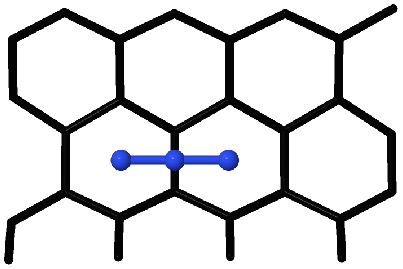
\includegraphics[width=\textwidth]{n3_t553_start_b-cropped.pdf}
        \caption{bond}
    \end{subfigure}
    \hspace{1cm}
    \begin{subfigure}{3cm}
        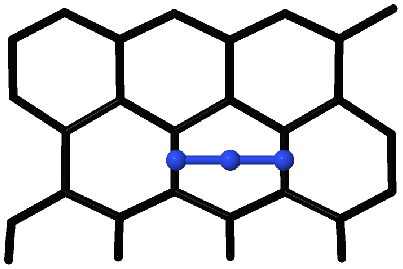
\includegraphics[width=\textwidth]{n3_t553_start_h-cropped.pdf}
        \caption{hollow}
    \end{subfigure}
    \hspace{1cm}
    \begin{subfigure}{3cm}
        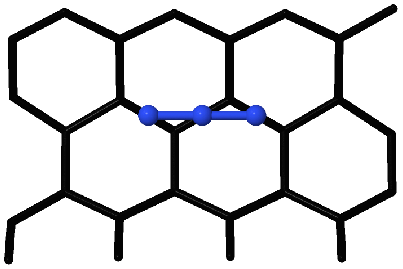
\includegraphics[width=\textwidth]{n3_t553_start_z-cropped.pdf}
        \caption{zigzag}
    \end{subfigure}
    \caption{Starting sites of the bond, hollow and zigzag geometries, respectively.}
}

\bfig{fig:n3t553_start_center}{
    \centering
    \begin{subfigure}{3cm}
        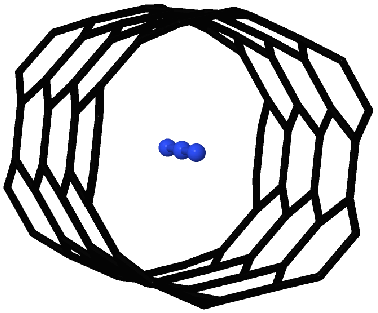
\includegraphics[width=\textwidth]{n3_t553_start_c-cropped.pdf}
    \end{subfigure}
    \hspace{1cm}
    \begin{subfigure}{3cm}
        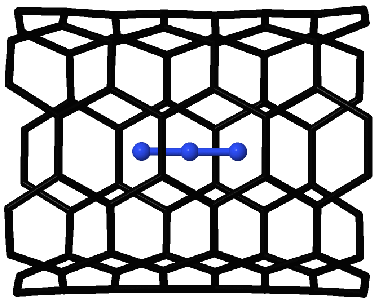
\includegraphics[width=\textwidth]{n3_t553_start_c_side-cropped.pdf}
    \end{subfigure}
    \caption{Central starting geometry (c). Note that the nanotube model has dangling hydrogen atoms at the two ends which are not shown here.}
}

\bfig{fig:n3t553_geom_parms}{
    \centering
    \begin{subfigure}{4.7cm}
        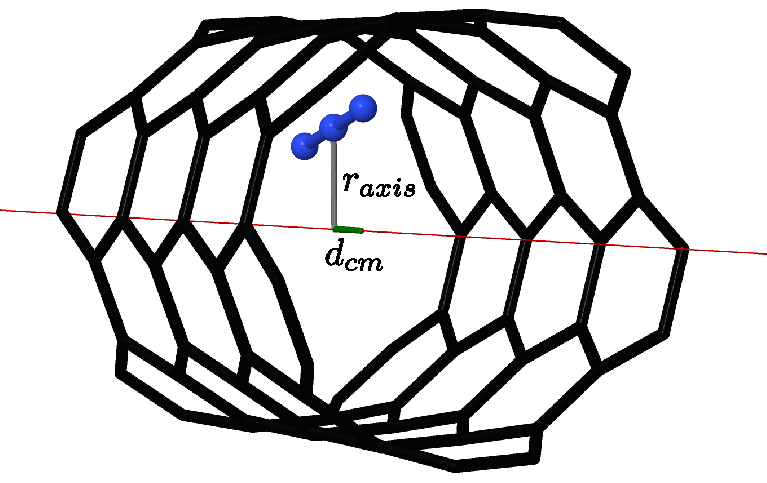
\includegraphics[width=\textwidth]{n3_t553_dist-cropped.pdf}
    \end{subfigure}
    \hspace{1cm}
    \begin{subfigure}{4cm}
        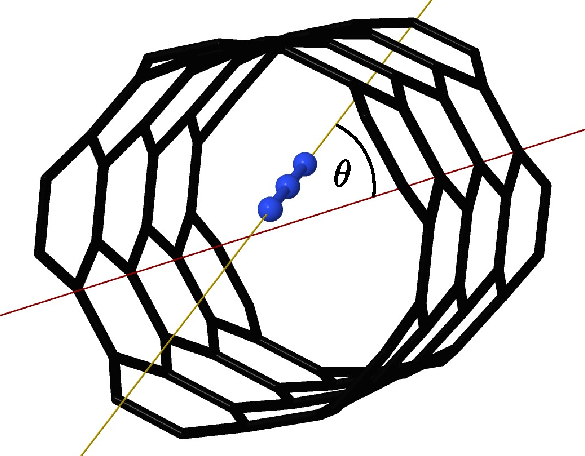
\includegraphics[width=\textwidth]{n3_t553_angle-cropped.pdf}
    \end{subfigure}
    \caption{Geometrical parameters.}
}
